\chapter{序論}
\label{chap:intro}

%----------------------------------------------
\section{本論文の背景}
%----------------------------------------------

音源分離とは,観測したある混合音源から,混合前の信号を推定する技術である.
この技術の具体的な応用例をFig.~\ref{fig:apps}に示す.
音源分離の例として音声信号に対する分離が挙げられる.
一例ではあるが,音声信号に対する分離では,混合信号から雑音を除去して音声だけを抽出及び強調するタスクや,複数人が会話を行っている状況下で個人毎に分離するような音声同士の分離タスク,\red{楽器音の自動採譜タスク}などがある.
近年では,スマートスピーカーのような音声認識技術を用いた製品が増えている中で,雑音や非目的話者の音声信号等の混合に起因した音声認識精度の低下を回避するためにも,目的話者のみのクリアな単一音声信号が入力として求められている.
音声認識だけでなく,イヤホンのノイズキャンセリング機能や補聴器の音声強調機能のように,人間の聴覚機能をサポートする面でも音源分離の応用先は数多く存在する.
%%%%%%%%%%%%%%%%%%%%%%%%%%%%
\begin{figure}[t]
    \vspace{4pt}
    \begin{center}
        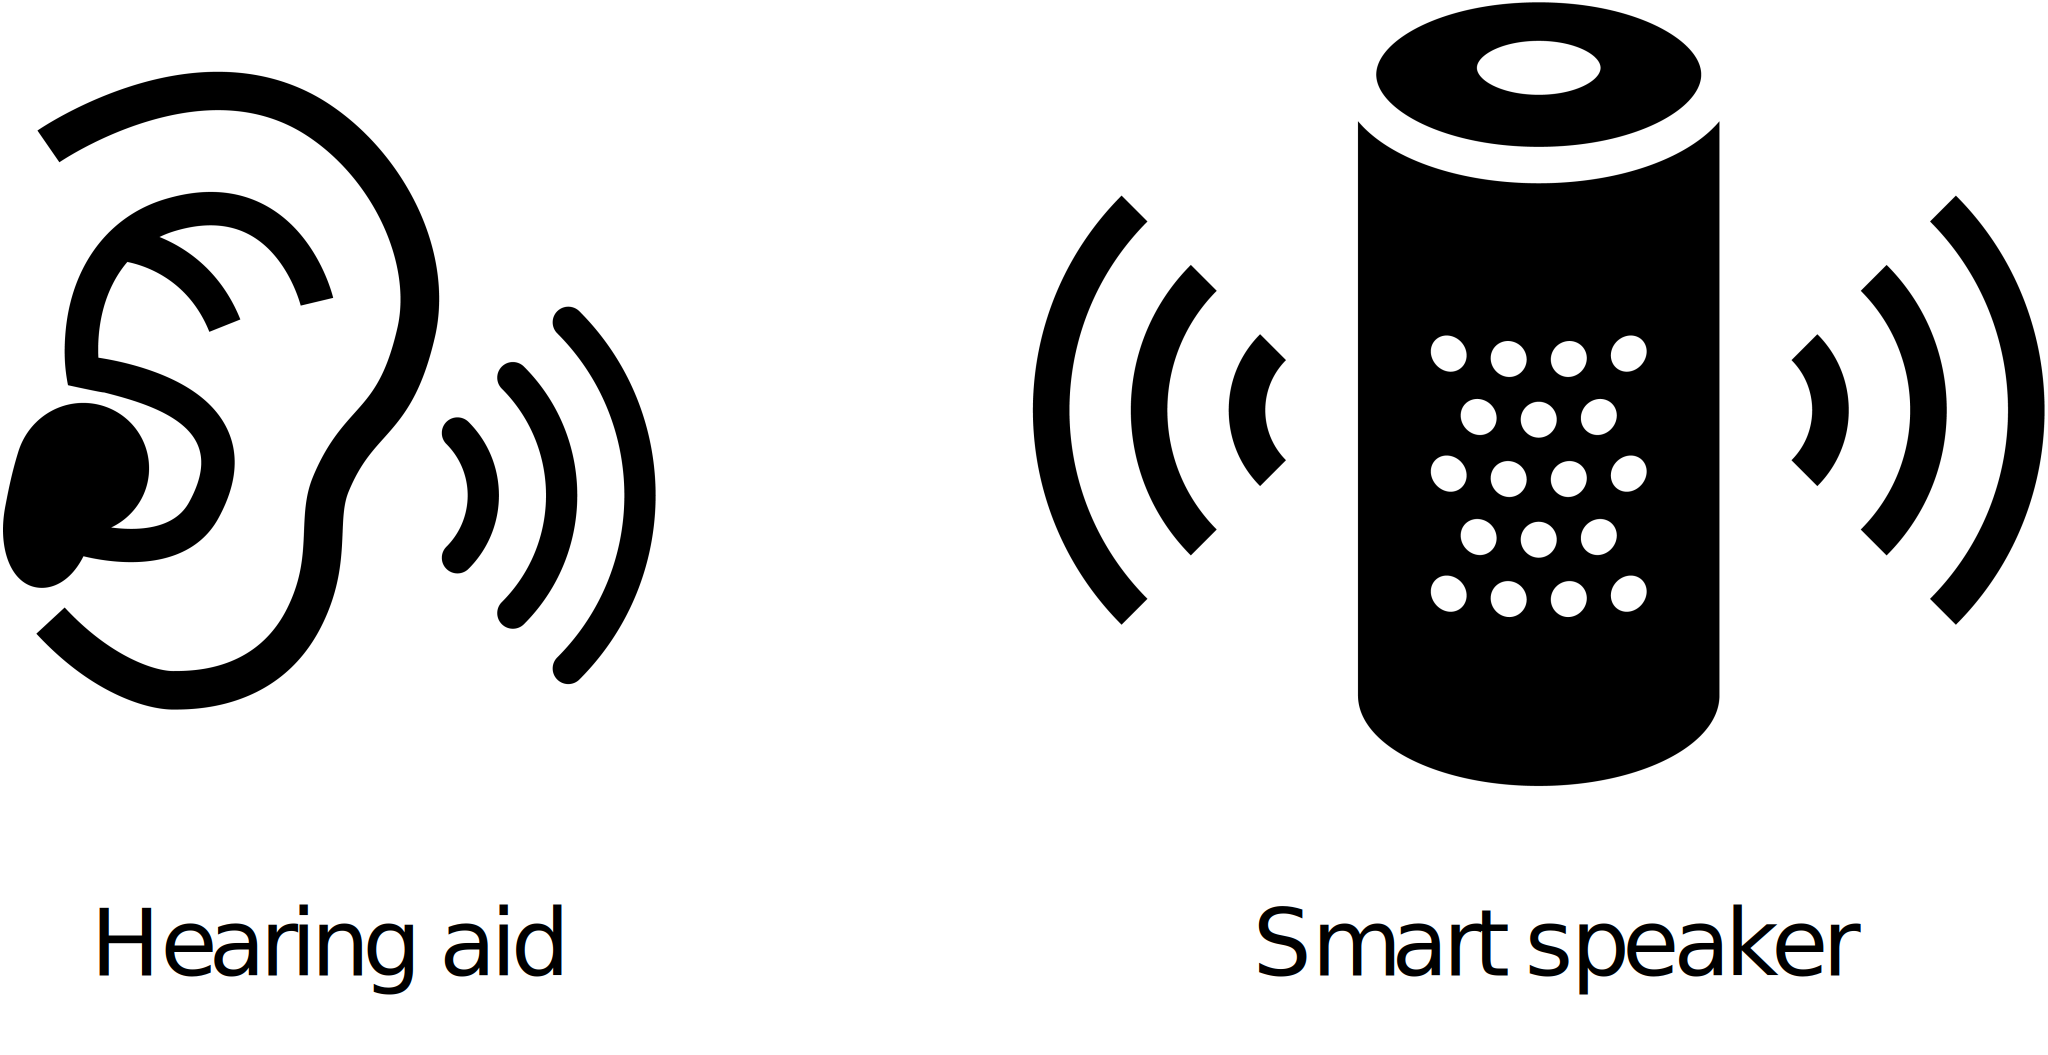
\includegraphics[width=0.7\columnwidth]{figures/using_audio_sep.pdf}
    \end{center}
    \vspace{-8pt}
	\caption{Examples of application using speech source separation.}
	\label{fig:apps}
\end{figure}
%%%%%%%%%%%%%%%%%%%%%%%%%%%%

上記のように,音源分離技術は\blue{近年ニーズが高まっており}\red{歴史的にみても非常に重要な技術として長年研究されており},これらのタスクを満足するには高精度な音源分離手法が求められる.
この経緯から1990 年代から今日まであらゆる音源分離手法が提案されてきた.
その音源分離手法の中でも,マイクロホンや音源の位置等の事前情報
が無いという条件下で,複数の信号源が混合した混合音から,混合前の分離音を推定するような分離手法をブラインド音源分離(blind source separation: BSS)\cite{BSS}という.
Fig.~\ref{fig:bss} はBSSの概要を示しており,未知の混合系$\bm{A}$(マイクロホンや音源位置や部屋の形状及び材質などに依存して変化)から混合信号が生成される.これに対して混合系$\bm{A}$の逆系である分離系$\bm{W}$を推定し,
\blue{混合系{$\bm{A}$}}観測信号$\bm{X}$に適用することで混合前の音源を推定する.
%%%%%%%%%%%%%%%%%%%%%%%%%%%%
\begin{figure}[t]
    \vspace{4pt}
    \begin{center}
        \includegraphics[width=0.9\columnwidth]{figures/BSS.pdf}
    \end{center}
    \vspace{-8pt}
	\caption{Overview of BSS.}
	\label{fig:bss}
\end{figure}
%%%%%%%%%%%%%%%%%%%%%%%%%%%%

特に,観測マイクロホン数が音源数以上となる\red{収録条件のことを優決定条件と呼ぶ.この条件下での}音源分離には,音源信号間の統計的独立性の仮定に基づく手法が広く用いられている.
独立成分分析(independent component analysis: ICA)\cite{ICA}は,優決定条件下の\red{BSS}に広く適用されている代表的な手法である.
音響信号の混合問題では一般的に残響の影響を受けて,瞬時混合ではなく時間畳み込み混合となることから,直接ICAを時間領域の観測信号に適用してもBSSを達成することは不可能である.
そこで,観測信号を時間周波数領域に変換することで周波数毎の瞬時混合として混合系をモデル化し,周波数毎にICAを適用する\red{時間}周波数領域ICA(frequency-domain ICA: FDICA)\cite{FDICA}が提案された.
ここで,ICAは一般に推定分離信号の順番が不定であり,FDICAは周波数毎に独立なICAによるBSSを行うため,分離信号の順番が周波数毎にばらばらになってしまう問題が生じる.
FDICAにおいて,周波数毎の分離信号を正しい順番に並び替える問題は一般に\red{「パーミュテーション問題」}と呼ばれており,過去には隣接周波数の時系列強度(音源アクティベーション)の相関を用いたパーミュテーション解決法\red{~\cite{COR,Permutation_solverBSS}},
マイクロホンの相対的な位置情報を既知として音源到来方位を計算し,パーミュテーション解決の手掛かりとする手法~\cite{DOA},及びその両者を組み合わせた手法~\cite{DOACOR}が提案されている.
また,近年ではFDICAに対して音源の時間周波数成分の共起関係を新たに仮定して,パーミュテーション問題を可能な限り回避しながら周波数毎の分離信号を推定する手法が登場している.
例えば,独立ベクトル分析(independent vector analysis: IVA)\cite{IVA1,IVA2}は,同一音源の周波数成分の共起を仮定しており,
非負値行列因子分解(nonnegative matrix factorization: NMF)\cite{NMF}とIVAを組み合わせた独立低ランク行列分析(independent low-rank matrix analysis: ILRMA)\cite{ILRMA1,ILRMA2}は同一音源の時間周波数成分の共起が低ランク構造を持つことを仮定している.


%----------------------------------------------
\section{本論文の目的}
%----------------------------------------------
前述したブラインドな音源分離手法は,パーミュテーション問題を回避しつつ,高い精度で分離するモデルへと発展を遂げてきた.
しかしながら,パーミュテーション問題の解は組み合わせ爆発を起こすことから,上記いずれの手法を用いても完璧にパーミュテーション問題を解くことは非常に難しい.
特に複数音声の混合信号や,\red{複数の調波楽器音の混合信号}における\red{頑健・}高精度なパーミュテーション問題の解決はいまだできていない.
一方で,文献~\cite{EU}では,複数音声の混合信号の分離時に正解のパーミュテーションを与えたFDICAが,ブラインドなIVAやILRMAよりも非常に高い分離精度を達成することを実験的に示している.
\red{従って,FDICAにおいて各周波数での音源分離は高精度であり,パーミュテーション問題のみが課題として残っている.}
\red{近年では,パーミュテーション問題を解決するために,深層ニューラルネットワーク(deep neural networks: DNN)を用いてサブバンドと呼ばれる局所帯域毎に,隣接した周波数のアクティベーションの相関を調べる手法~\cite{DNN_soluver}が提案されてきた.
しかし,この手法は局所帯域毎に処理をしているため,複雑なアルゴリズム構成となっており,3音源以上の音源分離を行うことは現実的には難しい.}
そこで,本論文では,\red{でもアルゴリズムが複雑化しない,}DNNを用いたデータ駆動型(教師あり)パーミュテーション解決法(以後,深層パーミュテーション解決法と呼ぶ)について\red{提案し,その妥当性について実験的に調査する}.
同時に,ブロックパーミュテーション問題に対\red{する有効性についても調査する}.
この\red{提案手法と既存手法の位置関係の概念図を}をFig.~\ref{fig:scope} に示す.
本論文では,FDICAにおけるパーミュテーション問題のみに焦点を当てており,分離信号成分の正しいパーミュテーションを予測する様に学習したDNNを用いてパーミュテーション問題を解決することを目的とする.
ここでは,DNN優決定条件下での複数音声の混合を模倣した人工的なデータと実際の音声及び音楽信号に対して,深層パーミュテーション解決法を適用することを考える.

%なお,劣決定音源分離において周波数毎のフルランク空間相関行列を推定するBSS ~\cite{FULLRANK}等でもパーミュテーション問題を解く必要が生じるため,提案手法はFDICAだけでなく,他の手法におけるパーミュテーション問題にも適用できる.
%%%%%%%%%%%%%%%%%%%%%%%%%%%%
\begin{figure}[t]
    \vspace{4pt}
    \begin{center}
        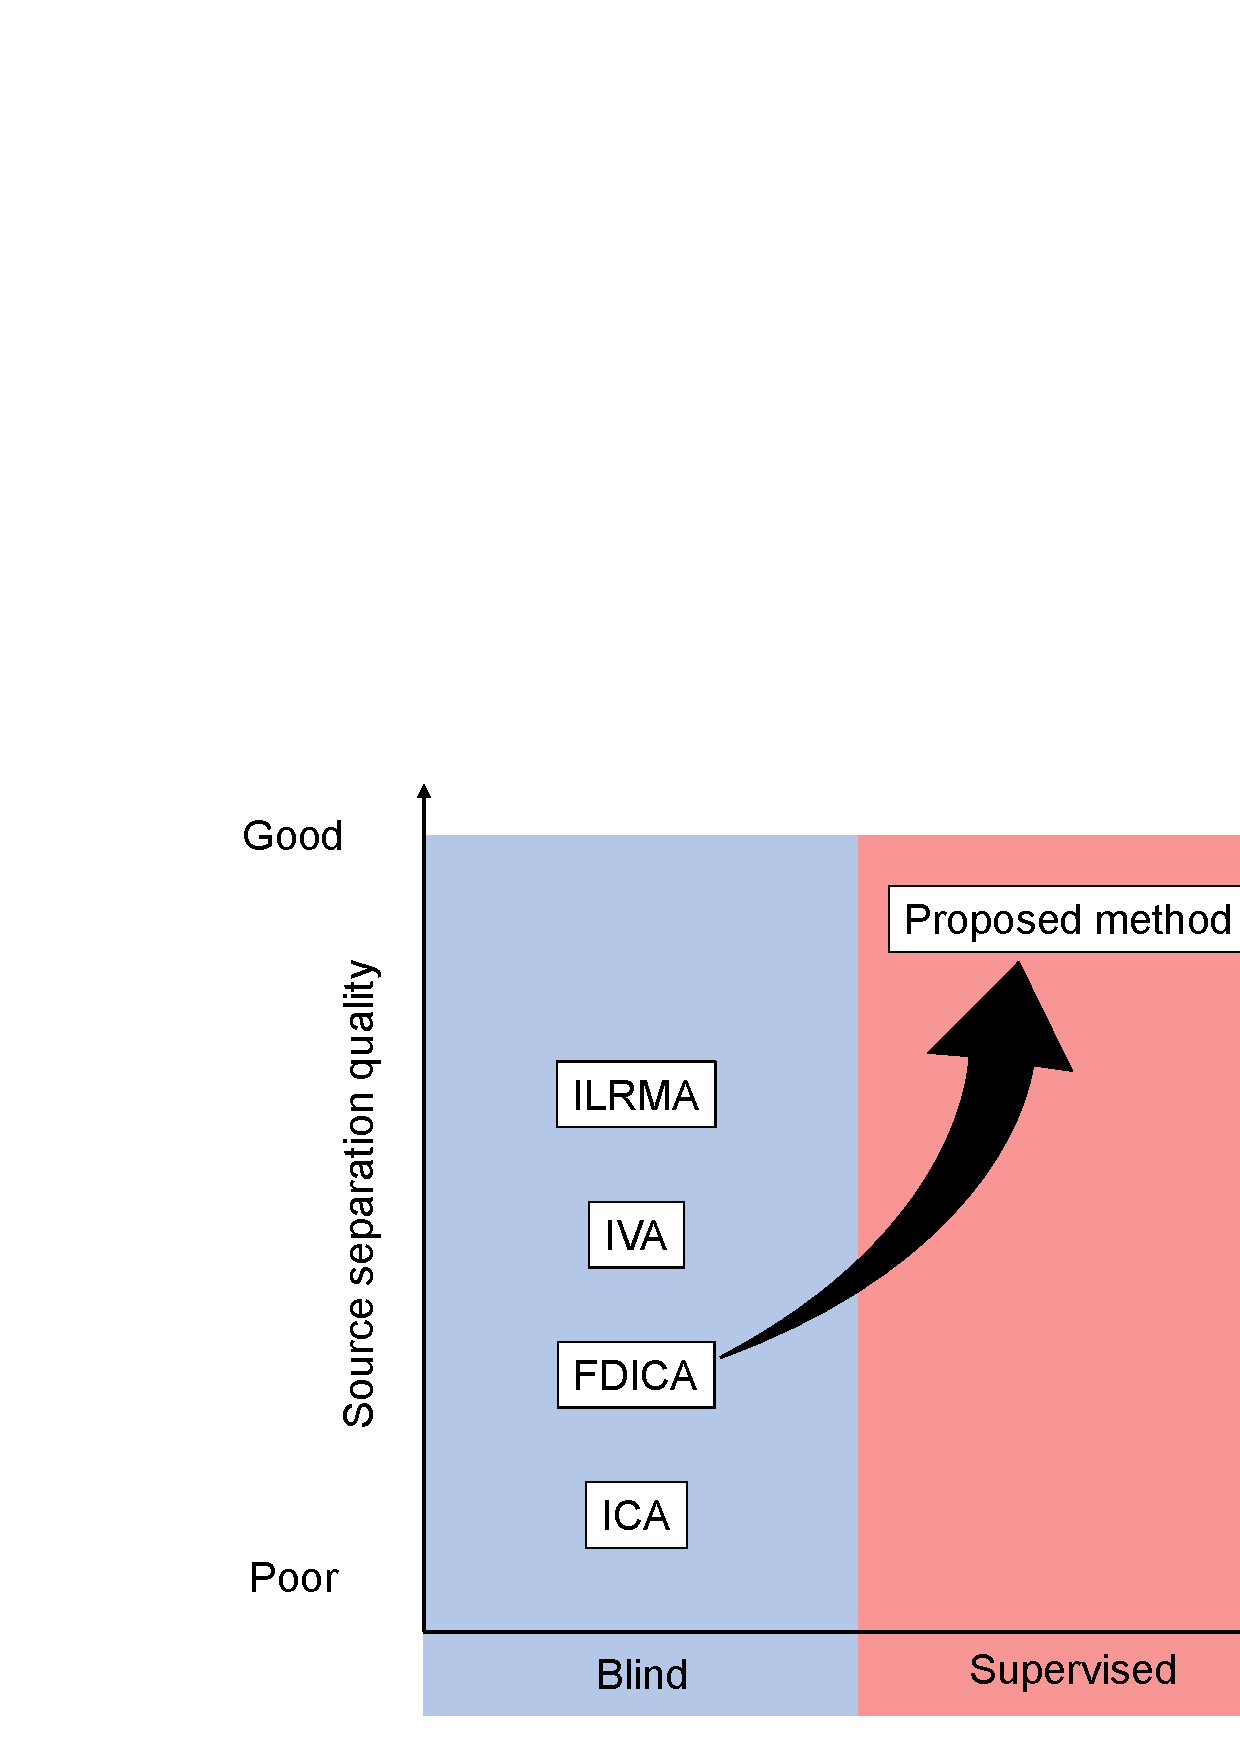
\includegraphics[width=1.0\columnwidth]{figures/chapter1/scope.pdf}
    \end{center}
    \vspace{-8pt}
	\caption{Scope of this thesis.}
	\label{fig:scope}
\end{figure}
%%%%%%%%%%%%%%%%%%%%%%%%%%%%


%--------------------------------------------
\section{本論文の構成}
%----------------------------------------------
まず,2章では,本論文の解決すべき課題であるパーミュテーション問題\red{の説明に必要となるICAの基本原理や音響信号の時間周波数領域への変換である短時間Fourier変換(short-time Fourier transform: STFT)に加え,
パーミュテーション問題を可能な限り回避するBSSのIVA及びILRMA,そして既存の深層パーミュテーション解決法について詳しく説明する.}
\red{これらは,いずれも提案手法の説明に必要となる知識である.}
3章では,本論文の提案手法である深層パーミュテーション解決法の新たなアルゴリズムの詳細について,\red{DNNの構造からパーミュテーション解決の処理までを詳細に述べる.}
4章では\blue{音声の混合信号を模倣した}人工データと実際の音声及び音楽信号に対する音源分離実験を行い,提案深層パーミュテーション解決法の性能の検証を行う.
最後に5章では, すべての章を総括した結言を述べる.


